\chapter{TiDAL: Visualizing Gene Regulatory Networks}
\label{chap:tidal}

\section{Purpose}

A software library is only useful if it can enhance or help produce better software applications.
Thus, the purpose of this chapter is to present the implementation of a Graphene application in visualizing the output of the bioinformatics tool, TiDAL (Time-Dependent Activity Linker).
This chapter supports the overall aims of this work by providing evidence of the utility of Graphene in producing interactive graphics for browser-based scientific tools.
The relative ease in which Graphene was integrated into an existing application demonstrates its flexibility and customizability, which also help support its scientific merit.

\section{Motivation}
\subsection{Pathogenic infections involve temporal regulatory cascades}

Pathogenic viruses, such as influenza and measles, subvert normal immune functioning through the expression of immune antagonists, such as the influenza NS1 protein. 
These antagonists differ between viral strains, and are crucial components of viral pathogenicity. 
Determining how these antagonists interact with the host immune system would be aided by knowledge of the genetic regulatory network that operates in response to infection. 


\subsection{High throughput data combined with computational methods may be used to infer regulatory transcription networks}



TiDAL \autocite{zaslavsky2013reconstruction} is a network reconstruction tool that takes time-series gene expression data and generates a transcription factor regulatory network.
TiDAL combines time-series expression kinetics and promoter sequence information to connect individual transcriptional regulators in a coherent, temporal, regulatory map. 

Briefly, the TiDAL works by processing gene expression data to determine differential expression, and then analyzing the differentially upregulated genes at each time point to derive time dependent profiles for each associated transcription factor.

TiDAL is available online (Figure \ref{fig:tidal-landing}). 
Users are free apply the algorithm to uploaded data set or publicly available one from InSilico DB \autocite{coletta2012insilico}.
TiDAL provides a valuable service by potentially allowing researchers to better interpret and understand their experimental results, which can shed light on the target pathobiology and identify possible interventions in disease.

\begin{figure}
  \centering
  \includegraphics[width=\textwidth,page=17,trim=0.37cm .65cm 0.37cm 0.3cm, clip=true]{images/Figures.pdf}
  \caption{TiDAL interface.}
  \label{fig:tidal-landing}
\end{figure}







\subsection{Temporal regulatory cascades are high dimensional and benefit from visualization}

TiDAL data is high dimensional because it involves connections between genes  and transcription factors, regulation among transcriptional factors, and the time axis.
To ease interpretation of the results, TiDAL provides several different forms of visualization (Figure~\ref{fig:tidal-output}), such as a heatmap (Figure~\ref{fig:tidal-output-heatmap}) and a table (Figure~\ref{fig:tidal-output-table}).

\begin{figure}
  \centering
  \begin{subfigure}[t]{0.3\textwidth}
    \includegraphics[width=\textwidth,page=18,trim=8.5cm 0cm 9cm 0cm, clip=true]{images/Figures.pdf}
    \caption{Heat map visualization of TiDAL output.
      The color scale correlates with upregulation of genes associated with transcription factor families (vertical axis) at time (horizontal axis).
    }
    \label{fig:tidal-output-heatmap}
  \end{subfigure}
  \begin{subfigure}[t]{.66\textwidth}
    \includegraphics[width=\textwidth,page=19]{images/Figures.pdf}
    \caption{Table view of TiDAL output.
      Similar to the heatmap representation, the table provides all numerical data points generated by TiDAL in connecting transcription factor activity over time.
    }
    \label{fig:tidal-output-table}
  \end{subfigure}
  \begin{subfigure}[b]{\textwidth}
    \includegraphics[width=\textwidth,page=20,trim=0.37cm 0.65cm 0.37cm 0.3cm, clip=true]{images/Figures.pdf}
    \caption{
      Graphene Network diagram of TiDAL output produced by Graphene.
      Transcription factors are represented as nodes and grouped by time activated.
      Edges indicate regulation between transcription factors.
      Red color edges indicate downstream regulation and green edges indicate upstream regulation.
      Upon  mouse hover over a node, its connect neighbors will be highlighted.
    }
    \label{Figure:tidal-output-graphene}
  \end{subfigure}
  \caption{Visualizations of TiDAL output.}
  \label{fig:tidal-output}
\end{figure}

\section{Solution}
\subsection{Network graph visualization of TIDAL output}

TiDAL uses Graphene for its network visualization (Figure~\ref{fig:tidal-output-graphene}).
Nodes in the diagram correspond to individual transcription factors.
Edges represent predicted regulatory relationships, are encoded as either feedforward (green), feedback (red), or reciprocal (black).
Time progresses vertically downward by each labeled subgraph. 
Nodes are placed within each subgraph in order by which the gene is first differentially expressed.
The node size is also scaled relative to the overall number of outgoing regulatory linkages, with larger nodes indicating higher connectivity.
Thus, the layout styling encodes additional dimensions of information to make interpretation of results easier for the user.

\subsection{User interaction for network exploration}

Since Graphene creates and binds the underlying result data directly to DOM elements, there are many possibilities for adding interactivity to the user interface that permits a greater level of data exploration.
Densely connected graphs may be difficult to interpret, thus on mouse hover over nodes, the diagram will dim all nodes and edges that are not the immediately connected to the target transcription factor.


\section{Implementation}
\subsection{Data binding with SVG template}

The entire source for the Graphene-TiDAL extension may be found online \autocite{gu2014grapheneTidal}.
A portion of the source will be abbreviated and presented here to discuss the implementation of Graphene-TiDAL.

The basal data object that drives SVG rendering is the output JSON from TiDAL that encapsulates the entire transcriptional regulatory network. 
The below is a truncated example of the JSON, which includes two nodes, each within a separate time slot, and one edge between.

\begin{lstlisting}[language=JavaScript]
{
  "nodes": [{
    "size": 341,
    "label": "TF",
    "id": 0,
    "name": "FOSL1"
  }, {
    "size": 174,
    "label": "TF",
    "id": 1,
    "name": "SREBF2"
  }, ],
  "edges": [{
    "nodes": [
      1,
      0
    ],
    "type": "prb"
  }],
  "timeSlots": {
    "2 hours": [
      0
    ],
    "4 hours": [
      1
    ]
  }
}
\end{lstlisting}

The fields \texttt{nodes}, \texttt{edges}, \texttt{timeSlots} are arrays of objects that comprise the entire network.
Within \texttt{nodes}, \texttt{id} is a number that uniquely identifies the node, which may be used by other objects to specify a particular node. 
The \texttt{size} attribute is the calculated measure of connectedness for that node, and \texttt{name} is the name of the transcription factor the node represents.

Within \texttt{edges}, each edge has the property \texttt{nodes}, which is an array of node identifiers, that specifies the source node in the first position and the target node in the second position.
The \texttt{type} property is a string value that can either be \texttt{“pr”}, indicating a feedforward effect, or \texttt{“prb”}, indicating a feedback effect.

Within \texttt{timeSlots}, each property is a time point value, which is an array containing the ID numbers for all nodes within it.

The TiDAL data controller (Appendix~\ref{appendix-tidal-dataCtrl}) watches for new JSON data, uses the D3 Barnes-Hut force directed layout algorithm to automatically lay out nodes, and exposes the data objects for rendering with the template.

The template is an HTML file that is contains with special annotations and directives that renders an in-memory data object into a DOM elements.

The below is a portion of the template file followed by a discussion on the view logic it encapsulates.

\begin{lstlisting}[language=html]
<g>
  <line
    ng-attr-stroke="{{{'prb': 'green', 'pr': 'red'}[link.type]}}"
    ng-attr-opacity="{{link.opacity || OPACITY.normal}}"
    ng-mouseover="mouseoverLink(link)"
    ng-mouseleave="mouseleaveLink(link)"
    ng-repeat="link in imports.edges"
    class="link"
    ng-attr-x1="{{link.x1}}"
    ng-attr-y1="{{link.y1}}"
    ng-attr-x2="{{link.x2}}"
    ng-attr-y2="{{link.y2}}"
    marker-end="url(#arrow)">
  </line>
</g>
<g ng-repeat="group in imports.groups">
  <g
    draggable
    ng-click="clickNode(node, $event)"
    ng-dblClick="dblClickNode(node, $event)"
    ng-mouseover="mouseoverNode(node, $event)"
    ng-mouseleave="mouseleaveNode(node, $event)"
    ng-attr-opacity="{{node.opacity}}"
    ng-repeat="node in group.nodes"
    class="node"
    ng-attr-transform="translate({{node.x}},{{node.y + $parent.$index * imports.subgraph.height}})">
    <rect
      ng-attr-x="{{-node.width/2}}"
      ng-attr-y="{{-node.height/2}}"
      ng-attr-width="{{node.width}}"
      ng-attr-height="{{node.height}}"
      ng-attr-ry="{{node.height / 2}}"
      fill="url(#gradient)">
        <title>ID: {{node.id}}, Name: {{node.name}}</title>
    </rect>
    <text class="node-label">{{node.name}}</text>
  </g>
</g>

\end{lstlisting}

One of the key components of the template is the \texttt{ng-repeat} directive, which is passed in an string expression that references an array object, with which the enclosing part of the DOM will be duplicated and appended for each item of the array. 
Statements within double curly braces, \texttt{\{\{value\}\}}, indicates an interpolated value from the scope of the enclosed DOM.

Within the \texttt{<line>} element, the \texttt{ng-repeat} attribute here specifies that a new \texttt{<line>} element is to be created from every value inside the \texttt{imports.edges} object, and for each new line to be bound to an reference to the edge item referred to as \texttt{link}.
The directive \texttt{ng-attr-*} indicates that the * attribute be added to the element and bound to the value of the interpolated object. Thus, each new \texttt{<line>} element will have x1, x2, y1, and y2 values equivalent to the corresponding item in the \texttt{edges} array. The layout controller (Appendix~\ref{appendix-tidal-layoutCtrl}) 


\subsection{Event handling}

\section{Future Directions}


